\documentclass[a4paper]{article}

\usepackage[italian]{babel}
\usepackage[utf8]{inputenc}
\usepackage{graphicx}
\usepackage{hyperref}

\begin{document}

\title{Risoluzione del problema STSP tramite metodo esatto e metaeuristica, comparazione}
%\subtitle{Relazione Progetto del corso di Metodi e Modelli per lOttimizzazione Combinatoria}
\author{Carlo Maria Massimo 1058513}
\date{\today}
\maketitle

\tableofcontents

    \section{Introduzione}
        Il lavoro in oggetto si propone lo scopo di valutare attraverso alcune sperimentazioni la bont\`a di metodi
        di risoluzione del problema STSP tramite metaeuristica rispetto a pi\`u collaudati metodi esatti.
        I metodi che sfruttano le metaeuristiche e qualche forma di ricerca locale sono spesso utilizzati per le migliori
        performance in termini di rapidit\`a di calcolo ed uso delle risorse, a fronte di un possibile degrado nella qualit\`a
        dei risultati forniti in output.

        In questo lavoro \`e stata implementata una ricerca tramite modello PLI con risolutore CPLEX ed una ricerca tramite algoritmo genetico.

    \section{Implementazione}
        L'implementazione della ricerca tramite metodo esatto \`e stata realizzata prendendo spunto da un'esercitazione di laboratorio
        relativa ad un problema di ATSP ed implementando in pratica il modello descritto nella consegna dell'esercitazione 1.

        L'implementazione della ricerca tramite algoritmo genetico \`e stata realizzata partendo dalla descrizione dei passi
        sulle dispense del corso, cercando per quanto possibile di introdurre qualche elemento di originalit\`a e di miglioramento rispetto
        allo schema standard dell'algoritmo proposto.

        \subsection{Note implementative}
        Durante gli esperimenti entrambe le ricerche partono da un'istanza del problema comune, modellata nella classe \emph{Instance}.
        Un oggetto della classe \emph{Instance} rappresenta il grafo dei fori che dovranno essere effettuati sulla piastra.
        In particolare \`e descritta da:

        \begin{enumerate}
            \item cardinalit\`a dell'insieme dei nodi del grafo (numero di fori)
            \item dimensioni della piastra (limite alle coordinate dei punti)
            \item la matrice delle distanze tra i nodi
            \item la lista dei nodi (identificati dalle proprie coordinate nello spazio 2D)
        \end{enumerate}

        La classe \emph{Model} racchiude il modello e la ricerca tramite PLI mentre le classi \emph{Solution}, \emph{Population} e \emph{Solver}
        implementano l'algoritmo genetico.

    \section{Risoluzione tramite modello PLI}
        Per risolvere il problema tramite modello di programmazione lineare intera mista si \`e ricorsi alla modellazione dello stesso come problema di
        rete di flusso e si \`e utilizzato il risolutore CPLEX per la ricerca di una soluzione ottima.
        Il modello implementato \`e quello fornito nell'esercitazione 1, la verifica della correttezza \`e stata fatta mediante ispezione del file
        \emph{stsp.lp} generato dal risolutore.

        \subsection{Il modello}
        
        La classe \emph{Model} contiene la definizione del modello per il problema, la modellazione implementata si discosta dall'approccio tradizionale che prevede la definizione di
        un problema di assegnamento con vincoli di subtour elimination.
        Modellando il problema come rete di flusso, si ottiene un modello con vincoli pi\`u semplici ed in numero nettamente inferiore.

        Si noti che, essendo il grafo che modella l'insieme dei fori un grafo completo, tra le variabili del modello che indicano la quantit\`a di flusso utilizzata ($x_{ij}$)
        vengono inserite nel modello anche le variabili relative ai cappi di ogni nodo ($x_{ij}$ con $i = j$).

        A questi archi viene associato un costo nullo in quanto si presume che la punta diamantata non sostenga alcun costo per rimanere ferma nello stesso punto; in virt\`u di questo
        anche se questi archi vengono inseriti nella soluzione risultano ininfluenti nel calcolo della funzione obiettivo.
        

    \section{Risoluzione tramite algoritmo genetico}
        L'algoritmo genetico implementato segue il seguente schema:
        \begin{enumerate}
            \item codifica delle soluzioni del problema;
            \item inizializzazione di una popolazione iniziale;
            \item ripetizione fino al soddisfacimento di condizioni di arresto:
                \begin{enumerate}
                    \item selezione coppie di parent dalla popolazione corrente;
                    \item generazione della progenie tramite ricombinazione delle coppie di parent;
                    \item rinnovamento della popolazione corrente tramite selezione dei nuovi individui
                        tra quelli appena generati, sulla base della misura di fitness;
                \end{enumerate}
            \item restituzione della soluzione migliore generata.
        \end{enumerate}

        \subsection{Parametri e calibrazione}
            Tutti i paramtri sono stati calibrati tramite \emph{grid search} a partire da un insieme di combinazioni ipoteticamente plausibile.
            I parametri coinvolti nella calibrazione sono:
            \begin{itemize}
                \item $accept\_prob\ (AP)$ ovvero un valore di probabilit\`a che determina:
                    \begin{itemize}
                        \item l'accettazione diretta di nuove soluzioni generate per ricombinazione;
                        \item l'applicazione della mutazione per inversione piuttosto che la rottura / riparazione della soluzione;
                    \end{itemize}
                \item $hc\_iterations\ (HCIT)$ che determina il numero di iterazioni massime nella ricerca locale;
            \end{itemize}

            La procedura di grid search ha calibrato questi due parametri in maniera differente per la fase di diversificazione (D) rispetto alla fase di intensificazione (I).

            All'interno della stessa procedura sono stati inoltre calibrati i parametri:
            \begin{itemize}
                \item $max\_tot\_iterations\ (MIT)$ che limita il massimo numero di popolazioni generabili dall'algoritmo;
                \item $iterations\_without\_improvement\ (ITWOI)$ che decide il limite di iterazioni improduttive (nelle quali la popolazione generata non apporta alcun miglioramento alla f.o.)
                    oltre il quale passare dalla fase di intensificazione alla fase di diversificazione;
                \item $pop\_size (PSZ)$ che determina la dimensione della popolazione.
            \end{itemize}

            Come accennato in precedenza si \`e partiti da un insieme di combinazioni di valori iniziale, si \`e quindi selezionata la combinazione con il miglior comportamento a fronte di 10 iterazioni
            di ricerca per un'istanza di problema (50 nodi fissi e coefficienti di costo fissati), da questa combinazione ne sono state derivate altre due variando leggermente alcuni parametri
            per ottenere effetti diversi e ne \`e stato studiato il comportamento sulla base di 10 iterazioni di ricerca su grafo fissato (50 nodi) con coefficienti di costo causali per osservarle
            in un ambiente pi\`u simile a quello degli esperimenti successivi.

            Dopo un leggero fine tuning dei valori le due combinazioni sono state mantenute entrambe e sono le seguenti:

            \begin{center}
                \begin{tabular}{|l|l|l|l|l|l|l|l|}  \hline
                    & $AP (D)$ & $AP (I)$ & $HCIT (D)$ & $HCIT (I)$ & $MIT$ & $ITWOI$ & $PSZ$ \\ \hline

                    C1 & 0.6        & 0.9        & 4       & 0           & 22000           & 10000            & 10    \\ \hline

                    C2 & 0.6        & 0.9        & 10       & 0           & 28000           & 10000            & 20    \\ \hline 
                \end{tabular}
            \end{center}


        \subsection{Codifica delle soluzioni}
            La codifica delle soluzioni adottata \`e quella detta ``path representation'', ovvero
            ogni soluzione \`e rappresentata da un vettore di interi (\emph{sequence}) che contiene
            gli indici del vettore dei nodi del grafo. L'ordine rappresentato nel vettore determina il cammino.
            Se la soluzione \`e ammissibile ogni indice appare solo una volta nel vettore \emph{sequence} e questo fa si che si riesca a modellare
            un ciclo hamiltoniano.

            La ricerca prevede la possibilit\`a di includere e generare soluzioni inammissibili all'interno di una popolazione.

        \subsection{Inizializzazione della popolazione iniziale}
            La popolazione di partenza viene generata nel modo seguente:
            \begin{itemize}
                \item met\`a di questa popolazione \`e generata scegliendo casualmente un indice tra 0 e la cardinalit\`a dei nodi per ogni elemento del vettore \emph{sequence} (soluzioni potenzialmente inammissibili);
                \item l'altra met\`a \`e generata permutando casualmente un vettore di indici univoci ordinati (soluzioni ammissibili).
            \end{itemize}
            Data questa popolazione, un'ulteriore passaggio ne seleziona casualmente una met\`a e la migliora tramite unsequencea
            ricerca locale di tipo \emph{Hill Climbing} che pu\`o essere o meno limitata nel numero di iterazioni
            dal fatto che si sia scelto di iniziare diversificando o intensificando la ricerca.

            La ricerca locale si basa su un vicinato 2-opt.

        \subsection{Selezione genitori}
            La fase di selezione degli individui per la ricombinazione procede selezionando dalla popolazione un certo numero
            (fissato) di coppie di individui distinti.
            La selezione avviene tramite la tecnica detta ``Fitness proportionate selection'', basandosi su una misura di \emph{fitness}
            definita come segue:

            $$f_i = (1 / e_i) - ic_i - hc_i$$

            dove:
            \begin{itemize}
                \item $e_i$ \`e il valore della funzione obiettivo sulla soluzione i-esima;
                \item $ic_i$ \`e il coefficiente di inammissibilit\`a definito proporzionalmente
                    al numero di ripetizioni nel vettore degli indici;
                \item $hc_i$ \`e il coefficiente di somiglianza con l'ottimo corrente definito proporzionalmente
                    all'inverso della distanza di Hamming con l'ottimo corrente se questa \`e maggiore di 0, un valore
                    fissato altrimenti.
            \end{itemize}

            Vengono create tante coppie quante sono gli individui di una popolazione.
        
        \subsection{Ricombinazione degli individui selezionati}
            Le coppie di individui parent cos\`i individuati vengono ricombinati tra di loro utilizzando l'operatore detto
            ``order-crossover''.

            Inizialmente si era optato per un operatore ``cut-point'' con $k$ punti di taglio definiti casualmente e variabili
            in numero tra una coppia e l'altra.
            Questo operatore \`e stato presto abbandonato in favore dell'``order-crossover'' in quanto causava un netto e veloce
            peggioramento delle soluzioni generate principalmente perch\'e estremamente inammissibili.

            Data l'inerente fragilit\`a di una soluzione nei confronti di operatori di ricombinazione insensibili rispetto ai nodi
            risultanti dalla ricombinazione si \`e preferito utilizzare l'operatore ``order-crossover'' che preserva l'ammissibilit\`a
            della soluzione generata rispetto ai genitori.

            Ogni nuova soluzione generata tramite ricombinazione, se ammissibile viene accettata con probabilit\`a $accept\_prob$,
            se inammissibile viene scartata con uguale probabilit\`a.
            Da questa procedura risulta una progenie di cardinalit\`a doppia rispetto a quella di una popolazione regolare.

            Gli individui di questo insieme vengono quindi sottoposti a mutazione ed in seguito a training.

            \subsubsection{Mutazione}
                Ogni individuo della progenie viene sottoposto, con probabilit\`a $accept\_prob$ ad un operatore di ``mutazione per inversione''.
                Nel caso in cui non gli venga applicato tale operatore l'individuo viene mutato comunque ma secondo il seguente schema:
                \begin{itemize}
                    \item se ammissibile: un gene selezionato casualmente viene impostato ad un valore casuale tra i possibili valori degli indici,
                        risultando quindi potenzialmente nella perdit\`a di ammissibilit\`a;
                    \item se inammissibile: viene ``riparato'', ovvero ogni ripetizione di indice viene sostituita con uno degli indici mancanti in maniera ordinata,
                        ripristinando l'ammissibilit\`a.
                \end{itemize}

                Si noti come questa secondo tipo di mutazione incida decisamente di pi\`u in fase di diversificazione in quanto $accept\_prob$ diminuisce.

            \subsubsection{Training}
                Conseguentemente alla fase di mutazione gli individui vengono migliorati tramite la stessa ricerca locale utilizzata per inizializzare
                la popolazione iniziale (\emph{Hill Climbing}).

                Anche in questo caso le iterazioni che l'algoritmo esegue sono limitate o meno a seconda che ci si trovi in fase di diversificazione o di intesificazione.

        \subsection{Rinnovamento della popolazione}
            Gli individui cos\`i manipolati vengono sottoposti quindi a selezione tramite ``Fitness proportionate selection'' fino a coprire la
            cardinalit\`a degli individui di una popolazione.

            La popolazione cos\`i ottenuta diviene la nuova generazione.
            
            Viene quindi confrontata la miglior soluzione della nuova generazione con l'ottimo corrente e se i criteri di arresto sono soddisfatti viene ritornata la migliore delle due soluzioni,
            altrimenti si procede con un'altra iterazione.
\newpage
    \section{Risultati delle simulazioni}
        
        \subsection{Esperimenti}
        I parametri degli esperimenti effettuati sono stati i seguenti:
        \begin{description}
            \item[E1] insieme dei nodi di cardinalit\`a 10--70 con step 10, inizializzazione casuale dei punti e dimensioni di piastra fissate (800x800);
            \item[E2] insieme dei nodi di cardinalit\`a 10--70 con step 10, inizializzazione casuale dei punti e dimensioni di piastra molto ridotte: 400x16;
            \item[E3] insieme dei nodi di cardinalit\`a 10--50 con step 10, inizializzazione casuale dei punti all'interno di 4 aree fissate (200x200) dopo aver suddiviso il piano (800x800) in 4 quadranti;
            \item[E4] insieme dei nodi di cardinalit\`a 10--70 con step 10, inizializzazione dei punti su una circonferenza e dimensioni di piastra fissate (800x800).
            \item[E5] insieme dei nodi di cardinalit\`a 100, inizializzazione casuale dei punti e dimensioni di piastra fissate (800x800).
        \end{description}

        \subsection{Risultati}
            Seguono i risultati ottenuti dalle simulazioni effettuate.
            \subsubsection{Ricerca con metodo esatto}

                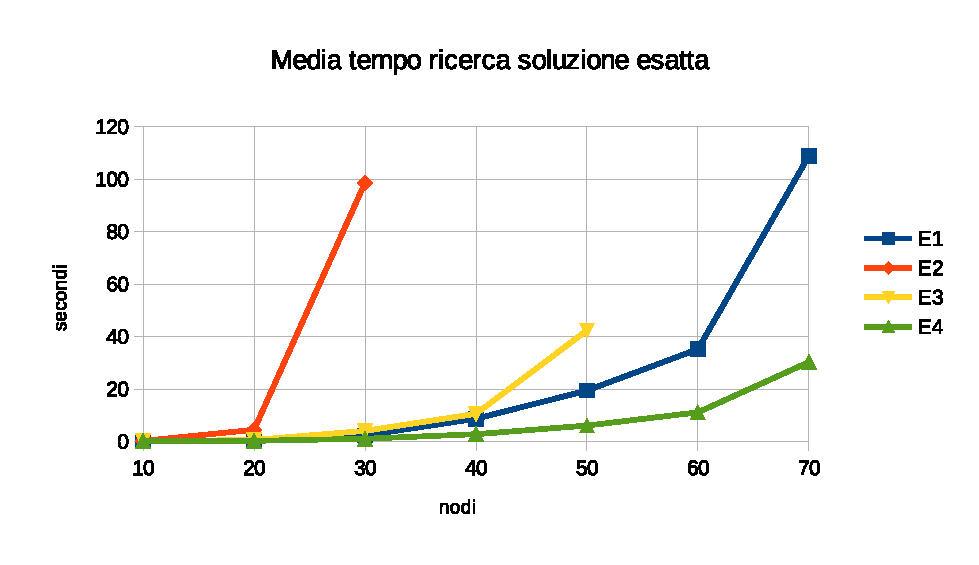
\includegraphics[scale=0.7]{img/exavgtime}

                I tempi di ricerca tendono a crescere esponenzialmente con l'aumento della cardinalit\`a dell'insieme dei nodi.
                Come facilmente prevedibile la conformazione del grafo incide pesantemente sulle performance del risolutore, con l'esperimento \textbf{E4} (fori su una circonferenza) che non eccede
                mai i 30 secondi e gli esperimenti \textbf{E2} (piastra molto piccola) ed \textbf{E3} (cluster) i cui tempi di ricerca crescono molto velocemente anche per dimensioni di problema molto piccole.


                \textbf{E5} si attesta su $496,04$ secondi.

                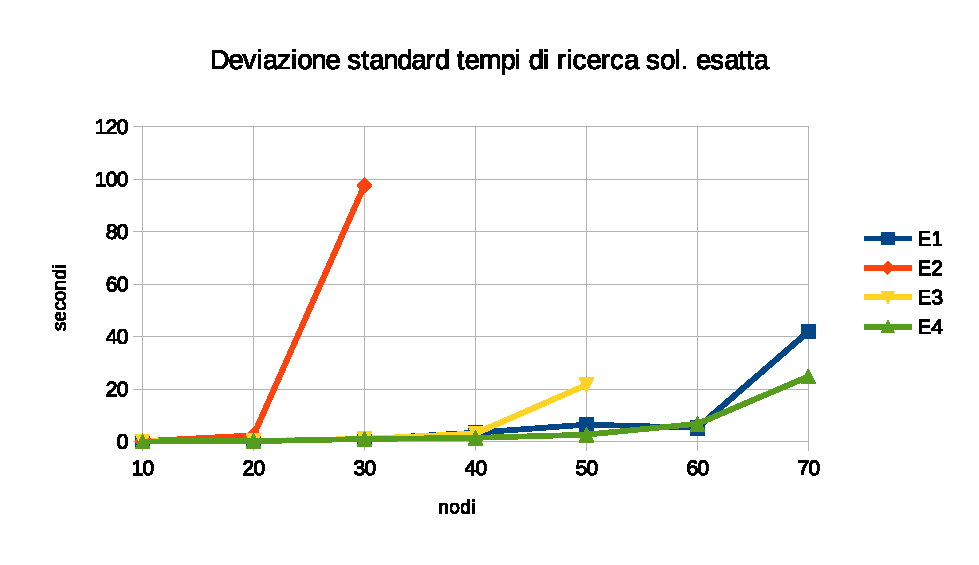
\includegraphics[scale=0.7]{img/exadevtime}

                La deviazione standard si mantiene contenuta a parte nei casi pi\`u complessi per ogni esperimento.

                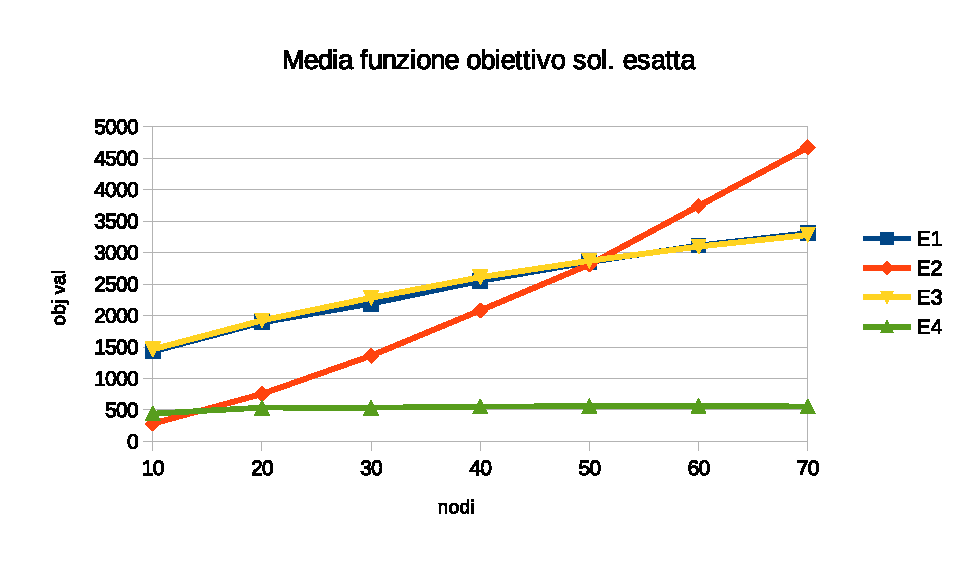
\includegraphics[scale=0.7]{img/exavgobj}

                
                La media della f.o. si mantiene praticamente costante in \textbf{E2} date le ridotte dimensioni di piastra e di nodi, in \textbf{E4} data la disposizione dei nodi del grafo che tendono sempre di pi\`u ad
                approssimare una circonferenza.

                Valore in \textbf{E5}: $6023,59$.

            \subsubsection{Ricerca con metaeuristica}

                    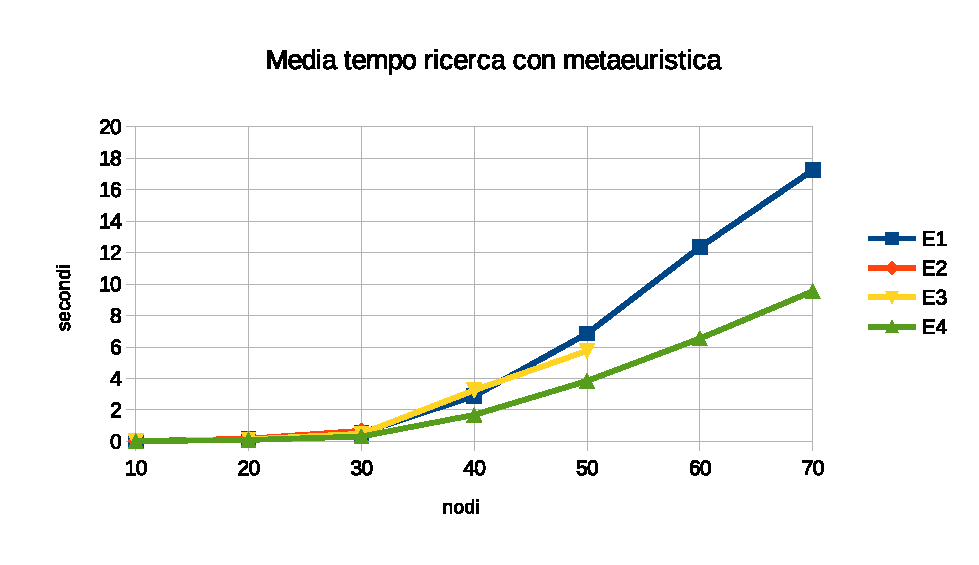
\includegraphics[scale=0.7]{img/gavgtime}

                    La crescita dei tempi di ricerca rispecchia esponenzialmente l'aumentare del numero di nodi fino alla dimensione 40 dove, si ricorda, entra in gioco un nuovo set di parametri di calibrazione della ricerca che volutamente incrementa (linearmente) il tempo dedicato alla ricerca di una soluzione pi\`u vicina all'ottimo.

                    I tempi rimangono comunque inferiori a quelli della ricerca esatta di quasi un ordine di grandezza.

                    Tempo impiegato in \textbf{E5}: $58,23$ secondi.

                    \includegraphics[scale=0.7]{img/gadevtime}

                    La deviazione standard dei tempi di ricerca rimane irrisoria nella maggior parte dei casi, salvo appunto nei problemi piu` complessi in termini di dimensioni.

                    \includegraphics[scale=0.7]{img/gavgobj}

                    La perdita di performance rispetto all'ottimalit\`a rimane estremamente contenuta.

                    In fase di calibrazione dei parametri di ricerca si \`e data priorit\`a al contenimento dei tempi di ricerca rispetto al miglioramento del valore della funzione obiettivo.

                    Il cambio di velocit\`a determinato dal differente set di parametri oltre la dimensione 30 \`e stato introdotto visto il corrispondente forte incremento dei tempi di ricerca del
                    risolutore CPLEX, e questo ha consentito una migliore approssimazione del risultato ottimo.

                    Valore in \textbf{E5}: $6576,51$.

                    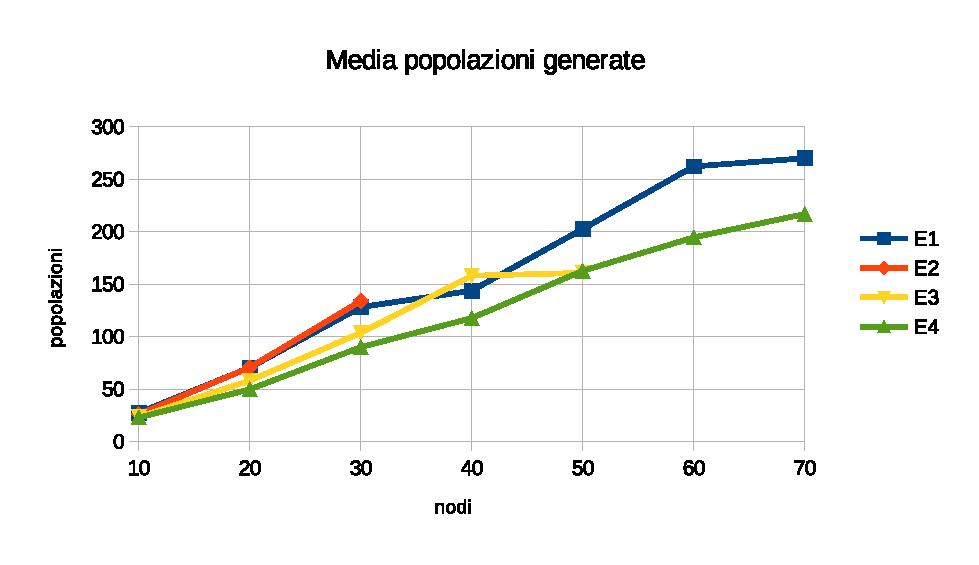
\includegraphics[scale=0.7]{img/popavg}

                    Il numero di iterazioni cresce abbastanza linearmente con l'aumentare della dimensione del problema fino a raggiungere un valore massimale in corrispondenza del problema con 30 nodi
                    dovuto al limite imposto al numero di iterazioni (popolazioni).

                    I valori riprendono a salire perch\'e il limite viene incrementato a partire dalla suddetta dimensione.  

                    In \textbf{E5}: 428 popolazioni in media.

                \subsubsection{Comparazione}

                    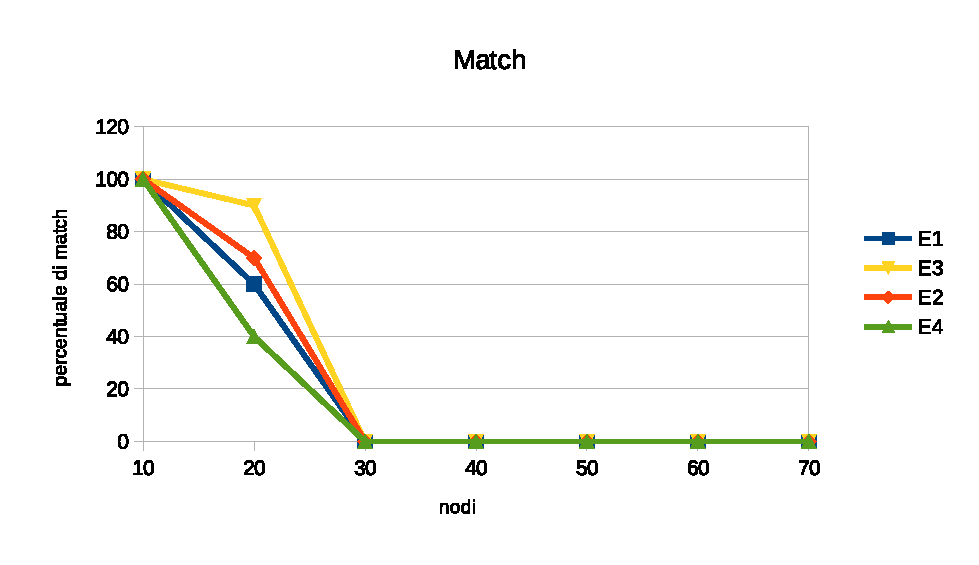
\includegraphics[scale=0.7]{img/match}

                    La ricerca con metaeuristica si comporta in maniera sostanzialmente molto simile alla ricerca con metodo esatto per dimensioni di problema modeste,
                    decrescendo nel numero di match man mano che il problema diviene pi\`u complesso.
                    
                    Come detto in precedenza si sono notati sostanziali miglioramenti per grafi con molti nodi aumentando il numero massimo di nuove generazioni permesse, perdendo qualcosa
                    in termini di tempi di risposta.

                    In \textbf{E5} non si \`e verificato match.

                    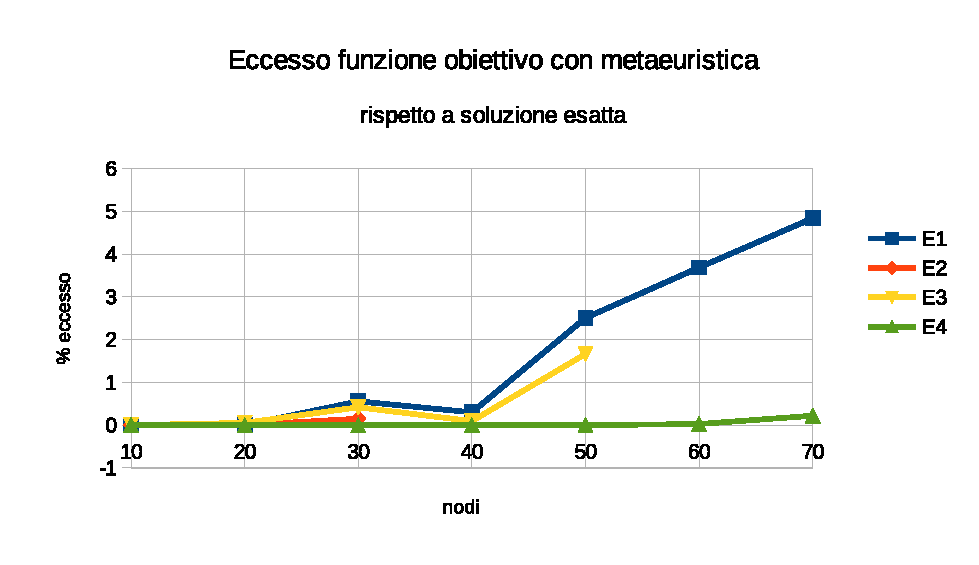
\includegraphics[scale=0.7]{img/excess}

                    Per quanto il grafico precedente mostri percentuali di match non molto elevate, si noti come l'eccesso del valore della f.o. restituito dalla ricerca con metaeuristica rispetto al valore
                    ottenuto con metodo esatto sia in realt\`a estremamente contenuto e non superi mai il $5\%$.

                    In \textbf{E5} l'eccesso \`e del $9\%$.

    \section{Conclusioni}
        STSP \`e un problema inerentemente molto complesso, che nel caso esatto richiede moltissimo sforzo.
        La ricerca nel caso esatto \`e inoltre piuttosto sensibile alla conformazione del problema, come involontariamente esemplificato
        dall'esperimento \textbf{E4}, mentre per contro la ricerca tramite metaeuristica sembra essere meno influenzata dalla struttura del grafo,
        a meno di casi estremamente particolari (la circonferenza di \textbf{E4} appunto).

        Con questo lavoro si \`e visto, non senza sorpresa, che \`e possibile raggiungere un buon grado di approssimazione rispetto ad una
        soluzione ottima, con tempi di esecuzione estremamente ridotti.

        \`E opinione dell'autore che un fine-tuning dei parametri di ricerca con adeguata strategia \emph{grid search} possa dare risultati
        ancora migliori rispetto a quelli esposti in questo documento.

\end{document}
